
\documentclass[12pt, french]{article}
\usepackage{fancyhdr, fancybox, lastpage, mathrsfs, tikz}
\usepackage[most]{tcolorbox}
\usepackage[a4paper, margin={0.3in, .75in}]{geometry}
\usepackage{wrapfig}
\pagestyle{fancy}
\renewcommand\headrulewidth{1pt}
\renewcommand\footrulewidth{1pt}
\fancyhf{}
\rhead{ \em{Zakaria Haouzan}}
\lhead[C]{\em{2ème année baccalauréat Sciences (Physiques + Mathématiques)}}
\chead[C]{}
\rfoot[C]{}
\lfoot[R]{}
\cfoot[]{\em{Page \thepage / \pageref{LastPage}}}


\newtcolorbox{Box2}[2][
enhanced, 
    breakable,
]{
                lower separated=false,
                colback=white,
colframe=white!20!black,fonttitle=\bfseries,
colbacktitle=white!30!gray,
coltitle=black,
enhanced,
attach boxed title to top left={yshift=-0.1in,xshift=0.15in},
title=#2,#1}


\begin{document}
\begin{center}
   \shadowbox {\bf{Les Systèmes mécaniques oscillants }
 }

\end{center}

\vspace{-0.2cm}
%%_________________________Exercice ! :"_________________________Exercice
   \begin{Box2}{Exercice 1 (2011SR): Etude d’un oscillateur mécanique.}

	\begin{wrapfigure}[11]{r}{0.26\textwidth}
  \begin{center}
	  \vspace{-0.6cm}
	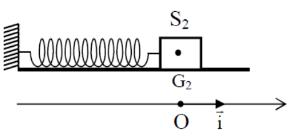
\includegraphics[width=0.26\textwidth]{./penduleElastique00.png}
	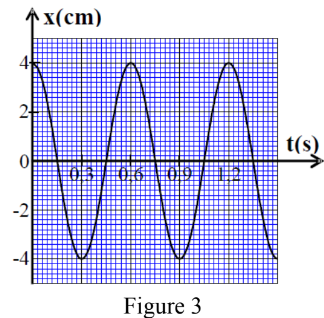
\includegraphics[width=0.26\textwidth]{./pendule_Elastique01.png}
  \end{center}
\end{wrapfigure}

\emph{On fixe à l’extrémité libre d’un ressort de masse
négligeable, à spires non jointives et de raideur K,
un solide (S2) de masse $m_2 = 182 g$. l’autre
extrémité est fixée à un support fixe (Figure 2).
Le solide (S2) est susceptible de glisser sur un plan
horizontal. }

On écarte le solide (S2) de sa position d’équilibre, d’une distance Xm, et on
l’abandonne sans vitesse initiale.
Pour étudier le mouvement du centre de gravité G2 du solide (S2), on choisit un repère
galiléen
(O,i), tel que G2 coïncide à l’équilibre avec l’origine O.
On repère la position de G2 à un instant t dans le repère

(O,i) , par son abscisse x.

L’équation différentielle du mouvement de G2
s’écrit sous la forme : $\ddot{x}$+$\frac{K}{m_2}.x = 0$, et sa solution
     est : $x(t) = X_m.cos(\frac{2\pi}{T_0}.t + \phi)$

     Une étude expérimentale a permis de tracer la
courbe représentée sur la figure 3.
\begin{enumerate}
  \item Déterminer graphiquement les
grandeurs suivantes :

    L’amplitude $X_m$, la période propre $T_0$ et la phase
$\phi$ à l’origine des dates.

\item En déduire la valeur de la raideur K du ressort.
\item On choisit comme état de référence de l’énergie potentielle de pesanteur, le
plan horizontal auquel appartient G2 à l’équilibre, et comme état de
référence de l’énergie potentielle d’élasticité, lorsque le ressort est non
déformé.
\begin{enumerate}
  \item Montrer que l’expression de l’énergie cinétique $E_C$ du solide $(S_2)$
    s’écrit sous la forme : $E_c = \frac{K}{2}.(X_m^2 - x^2)$.
  \item Trouver l’expression de l’énergie mécanique $E_m$ du système
{solide $(S_2)$ – ressort} en fonction de $X_m$ et K, et déduire la valeur de
    la vitesse $V_{G2}$ au passage de $G_2$ à la position d’équilibre dans le sens
positif.
\end{enumerate}
\end{enumerate}


   \end{Box2}


%%_________________________Exercice !2 :"_________________________Exercice
\begin{Box2}{Exercice 2 (2023SN):Etude du mouvement d’une balançoire }
   \begin{wrapfigure}[11]{r}{0.16\textwidth}
  \begin{center}
	  \vspace{-0.6cm}
	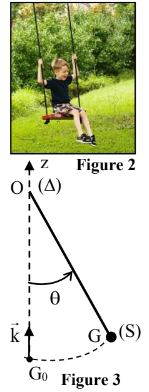
\includegraphics[width=0.16\textwidth]{./pendule_simple00.png}
  \end{center}
\end{wrapfigure}
Un enfant oscille à l’aide d’une balançoire (figure2).

  On modélise la balançoire avec l’enfant par un pendule formé par un corps solide (S) de
masse m et de centre d’inertie G , suspendu en un point O par une tige rigide, de masse
négligeable et de longueur pouvant effectuer un mouvement de rotation dans un plan
vertical autour d’un axe horizontal $\Delta$
passant par O (figure 3) . 

  On étudie le mouvement du pendule dans un repère $(G_0 ;\vec{k})$
lié à un référentiel terrestre supposé galiléen.

On écarte le pendule de sa position d’équilibre stable d’un angle petit $\theta_0 = 9^{\circ}$, dans le
sens positif, puis on le lâche sans vitesse initiale à l’instant de date $t_0 = 0$.
On repère la position du pendule à un instant de date t par l’abscisse angulaire $\theta$.
On néglige tous les frottements et on choisit le plan horizontal passant par
$G_0$ (position de G à l’équilibre stable) comme état de référence de l’énergie potentielle de pesanteur 

  $E_{pp} = 0$.



\textbf{Données : }
\begin{itemize}
  \item Le moment d’inertie du pendule par rapport à l’axe $(\Delta)$ est : $J_{\Delta} = ml^2$
  \item Accélération de la pesanteur $g = 10 m.s^{-2}$ ; $l = 2,4m$.
  \item Pour les oscillations de faible amplitude, on prend $cos(\theta) \approx 1 - \frac{\theta^2}{2} $; $\theta$ en radian.
\end{itemize}

\begin{enumerate}
  \item Montrer que l’expression de l’énergie potentielle de pesanteur du pendule à un instant t pour les
    oscillations de faible amplitude est : $E_{pp} = \frac{1}{2}.mgl\theta^2$.
  \item En exploitant la conservation de l’énergie mécanique du pendule :
  \begin{enumerate}
    \item Déterminer la vitesse angulaire maximale $\dot{\theta}_{max}$ du centre d’inertie G.
    \item Etablir l’équation différentielle du mouvement vérifiée par l’abscisse angulaire $\theta(t)$.
    \item Calculer la période propre de ce pendule sachant qu’il est analogue à un pendule simple de
longueur et $l$ de masse $m$.
  \end{enumerate}
\end{enumerate}

\end{Box2}

\begin{Box2}{Exercice 3 (2013SR): Etude du mouvement d’un pendule pesant. }
   
  \begin{wrapfigure}[11]{r}{0.2\textwidth}
  \begin{center}
	  \vspace{-0.6cm}
	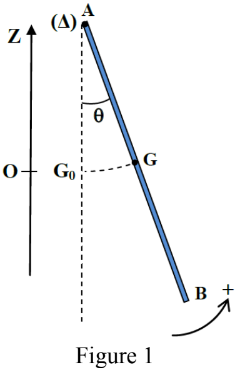
\includegraphics[width=0.2\textwidth]{./pendule_pesant00.png}
  \end{center}
\end{wrapfigure}
  \emph{L’homme a utilisé les hologes depuis longtemps, il a inventé plusieurs types tel que :
l’horloge solaire, l’horloge hydraulique, l’horloge à sable... jusqu’à ce que le savant
Huygens inventa l’horloge murale en 1657.
Le fonctionnement de cette horloge dépend de son balancier, qu’on modélise par un
pendule pesant, effectuant des petites oscillations libres sans frottements.}

Le pendule étudié est constitué d’une barre homogène
AB, de masse $m $=$0,203 kg$, et de longueur
$AB = l = 1,5 m$, susceptible de tourner dans un plan
vertical autour d’un axe horizontal $(\Delta)$, fixe et passant
par son extrémité A (figure 1).

On étudie le mouvement du pendule dans un repère lié à
la terre et supposé galiléen.

  On repère à chaque instant le pendule par son abscisse
angulaire $\theta$.

Le moment d’inertie de la barre par rapport à l’axe ($\Delta$)
  est : $J_{\Delta} = \frac{1}{3}.ml^2$

  On admet que dans le cas des petites oscillations que :
$sin\theta \approx \theta$ avec $\theta$ en rad. Figure 1
On désigne l’intensité de pesanteur par la lettre g.

On écarte le pendule de sa position d’équilibre stable d’un petit angle $\theta_m$ dans le sens
positif, et on le lâche sans vitesse initiale à un instant choisi comme origine des temps.
  \section*{1- Etude dynamique du pendule pesant :}
  \begin{enumerate}
    \item[1-1-] Par application de la relation fondamentale de la dynamique de rotation,
établir l’équation différentielle du mouvement du pendule.
\item[1-2-] Préciser la nature du mouvement du pendule pesant, et écrire son équation
horaire $\theta(t)$ en fonction de t, $\theta_m$ et la periode propre $T_0$.
\item[1-3-] Montrer que l’expression de la période propre $T_0$ est : $T_0 = 2.\pi.\sqrt{\frac{2.l}{3g}}$
\item[1-4-] Calculer la valeur de la longueur L du pendule simple synchrone au
pendule pesant étudié.
  \end{enumerate}

  \begin{wrapfigure}[4]{r}{0.4\textwidth}
  \begin{center}
	  \vspace{-1cm}
	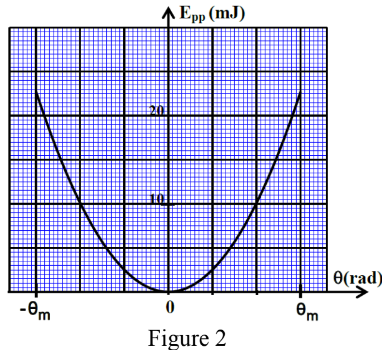
\includegraphics[width=0.4\textwidth]{./Energy_pendulepesant00.png}
  \end{center}
  \end{wrapfigure}

  \section*{2-Etude énergétique du pendule pesant : }

  On choisit le plan horizontal contenant le point G0, position du centre de gravité G de
la barre à la position d’équilibre stable, comme état de référence de l’énergie
  potentielle de pesanteur $(E_{PP} = 0)$.


La figure 2 représente les variations de
  l’énergie potentielle de pesanteur $E_{PP}(\theta)$
du pendule étudié dans l’intervalle $[-\theta_m, \theta_m]$
Par exploitation du diagramme d’énergie :
   \begin{enumerate}
     \item[2-1-] Donner la valeur de l’énrgie
mécanique $E_m$ du pendule.
\item[2-2-] Trouver la valeur absolue de la
vitesse angulaire $\dot{\theta}$ du pendule
au passage par la position
       repérée par l’abscisse angulaire : $\theta = \frac{2}{3}.\theta_m$
   \end{enumerate}
\end{Box2}



	%\vspace{-0.8cm}
\begin{center}
   \Large{ \em{Exercices Supplémentaires}}
\end{center}



\begin{Box2}{Exercice 4 (2009SR):Etude d’un oscillateur mécanique}

   
  \begin{wrapfigure}[11]{r}{0.2\textwidth}
  \begin{center}
	  \vspace{-0.6cm}
	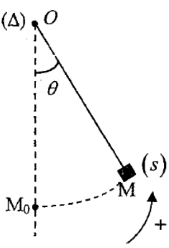
\includegraphics[width=0.2\textwidth]{./ps_01.png}
  \end{center}
\end{wrapfigure}

  \emph{Les oscillateurs sont utilisés dans plusieurs domaines d’industrie, et quelques
appareils de sport, de jeux et autres. Parmi ces oscillateurs, la balançoire considérée
comme pendule.}
Un enfant se balance à l’aide d’une balançoire constituée d’une barre utilisé comme
siège, suspendue à l’aide de deux câbles fixés à un support fixe.

On modélise le système {Enfant + Balançoire} par un pendule simple constitué d’un :
\begin{itemize}
  \item Câble inextensible, de masse négligeable, et de longueur l ;
  \item Solide (S) de masse m.
\end{itemize}
Le pendule est susceptible de tourner autour d’un axe horizontal fixe ($\Delta$)
perpendiculaire au plan vertical.

\textbf{Données : }
\begin{itemize}
  \item Le moment d’inertie du pendule par rapport à l’axe $(\Delta)$ est : $J_{\Delta} = ml^2$
  \item Accélération de la pesanteur $g = 10 m.s^{-2}$ ; $l = 3m$ ; $m = 18Kg$.
  \item Pour les oscillations de faible amplitude, on prend $cos(\theta) \approx 1 - \frac{\theta^2}{2} $; $\theta$ en radian.
  \item On néglige les dimensions de (S) par rapport à la longueur du fil, ainsi que tous les
frottements.
\end{itemize}
  \textbf{1. Etude dynamique du pendule :}
  On écarte le pendule de sa position d’équilibre d’un angle $\theta_m = \frac{\pi}{20}$ dans le sens

positif, et on l’abandonne sans vitesse initiale à l’instant $t = 0$.
On repère la position du pendule à un instant t par son abscisse
angulaire $\theta$ entre le pendule et la verticale passant par O, tel que $\theta = (\vec{OM_0}, \vec{OM})$

\begin{enumerate}
  \item[1-1-] Par application de relation fondamentale de la
dynamique de rotation autour d’un axe fixe, montrer
que l’équation différentielle du mouvement du
pendule dans un repère galiléen lié à la terre s’écrit
    sous la forme : $\ddot{\theta} + \frac{g}{l}\theta = 0$
  \item[1-2-] Calculer la valeur de la période propre $T_0$ du pendule.
  \item[1-3-] Ecrire l’équation horaire du mouvement du pendule.
  \item[1-4-] Par application de la deuxième loi de Newton, et sa projection sur les axes
du repère de Freinet, exprimer l’intensité T de la tension du câble à
l’instant t en fonction de : $m$, $g$, $\theta$, $l$ et $v$ (Vitesse linéaire du solide (S)).
    Calculer la valeur de T à l’instant $t = \frac{T_0}{4}$
\end{enumerate}
  \textbf{2. Etude énergétique :}
  On communique au pendule précédent initialement au repos à t = 0, une énergie
cinétique de valeur $E_C = 264,6 J$, qui le fait tourner dans le sens positif.
\begin{enumerate}
  \item Ecrire l’expression de l’énergie potentielle de pesanteur $E_{pp}$ du pendule à un
instant t en fonction de $\theta$, m, l et g.
\item Le plan horizontal passant par $M_0$ et choisi comme état de référence de l’énergie
potentielle de pesanteur.
A l’aide d’une étude énergétique, déduire la valeur maximale $\theta_m$ de
l’abscisse angulaire.

\end{enumerate}
\end{Box2}




\begin{Box2}{Exercice 5 : Pendule élastique vertical}

  \begin{wrapfigure}[6]{r}{0.2\textwidth}
  \begin{center}
	  \vspace{-0.6cm}
	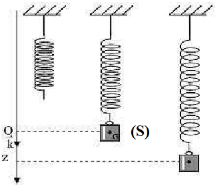
\includegraphics[width=0.2\textwidth]{./img/pevàà.png}
  \end{center}
\end{wrapfigure}

Un ressort a spires non jointives de masse  négligeable  de constante de raideur K est lié  a un corps (S), supposé
ponctuel et de masse m, qui peut se d´eplacer verticalement dans le champ de pesanteur terrestre. (voir figure
ci-contre ) .

On choisit comme origine de l'énergie potentielle de pesanteur la position d'équilibre O et comme origine de l'énergie potentielle elastique l'etat ou le ressort n'est pas allongé
  \begin{enumerate}
    \item Déterminer l’allongement $\Delta{l_0}$ du ressort dans la position
d’´equilibre du corps (S) .
\item Etablir l’´equation différentielle du mouvement de $(S)$
vérifié par sa position $z(t)$
\item Déterminer l'expression de l'énergie potentielle totale du système et calculer sa valeur dans la position d'équilibre
\item En déduire l'expression de l'énergie mécanique du système
\item Montrer que l’énergie mécanique du système se conserve et
  calculer la vitesse maximale $v_{max}$
\item Retrouver l’équation différentielle par méthode énergétique:
  \end{enumerate}
\end{Box2}


%\vspace{-0.8cm}

%%%_________________________Exercice ! 3:"_________________________Exercice
\begin{Box2}{Exercice 6: Pendule élastique deux ressorts}
%%\begin{wrapfigure}{r}{0.4\textwidth}
 %%\end{wrapfigure}
  \begin{wrapfigure}[4]{r}{0.2\textwidth}
  \begin{center}
	  \vspace{-0.6cm}
	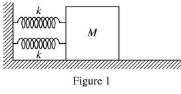
\includegraphics[width=0.2\textwidth]{./img/psh11.png}
  \end{center}
\end{wrapfigure}
  un solide S de masse $m = 800g$ est accroché à l’extrémité de deux ressorts identiques de constante de raideur
  $k = 40N/m$ (voir figure 1)
à la date t = 0s,on déplace le solide de sa position d’équilibre O sur l’axe horizontal OX dans le sens positif de
  $x_0 = 4cm$ et lui communique une vitesse initiale $v_0 = 0, 2m/s$ dans le sens négatif les frottements sont supposées
négligeables.
\begin{enumerate}
  \item appliquer la 2ème loi de Newton pour trouver l’équation différentielle vérifiée par l’abscisse $x(t)$
  \item Retrouver cette équation différentielle par conservation de l’énergie
mécanique $E_m$
\item Trouver les dates du passage du solide par l’origine en allant dans le sens
positif
\item  la solution de l’équation différentielle est : $x(t) = X_m.cos(\frac{2\pi t}{T} + \phi)$. Trouver $X_m$;$T$; et $\phi$
\end{enumerate}
\end{Box2}

%%_________________________Exercice 4 : _________________________Exercice
\begin{Box2}{Exercice 7 :oscillations}
   %% \begin{wrapfigure}[12]{r}{0.5\textwidth}
\begin{wrapfigure}[4]{r}{0.4\textwidth}
  \begin{center}
	  \vspace{-0.6cm}
	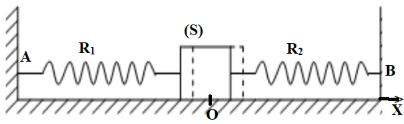
\includegraphics[width=0.4\textwidth]{./img/doublephe.png}
  \end{center}
\end{wrapfigure}

un solide S de masse $m = 200g$ est astreint à se mouvoir horizontalement sur un plan sans frottement à l’aide
     de deux ressort à spires non jointives de masses négligeable de longueur à vide $l_{01}$ et $l_{02}$ de raideurs respectives ;
     $k_1 $=$20N/m$ et $k_2$.( voir figure ) la distance $AB > l_{01} + l_{02}$.
\begin{enumerate}
  \item Etudier l’équilibre et en déduire la relation entre les allongement $\Delta{l_{01}}$ et $\Delta{l_{02}}$
  \item On écarte S de $x_0 = 2cm$ dans le sens positif et on lui communique une vitesse initiale $v_0 $=$-0, 2m/s$ à la
date $t = 0s$ . il effectue alors des oscillations rectiligne sinusoidales de période propre $T_0 = 4s$
\begin{enumerate}
  \item Montrer que l’équation différentielle vérifiée par l’abscisse x(t) est :$\ddot{x} + \frac{K_e}{m}x = 0$

    préciser l’expression de ke en fonction de $k_1$ et $k_2$.
  
\end{enumerate}
\item dans le dispositif qui suit, les ressorts sont de masses négligeable , de constantes de raideurs respectifs K1 et k2 et
la masse du corps $(S)$ est $m$ Trouver l’équation différentielle vérifiée par $x(t)$ par deux méthodes

\end{enumerate}
  \begin{center}
	  \vspace{-0.6cm}
	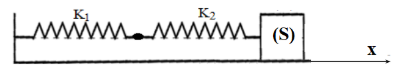
\includegraphics[width=0.4\textwidth]{./img/ph03.png}
  \end{center}

\end{Box2}

\begin{Box2}{Exercice 8 :Pendule élastique incliné}
   %% \begin{wrapfigure}[12]{r}{0.5\textwidth}
\begin{wrapfigure}[4]{r}{0.3\textwidth}

  \begin{center}
	  \vspace{-0.6cm}
	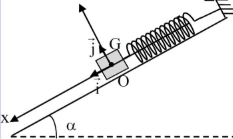
\includegraphics[width=0.3\textwidth]{./img/inclinee.png}
  \end{center}
\end{wrapfigure}
On considère le dispositif ci-contre où le ressort est à spires non jointives de masse négligeable de raideur K et le
solide (S) est considéré comme ponctuel de masse m à l’équilibre , il se trouve en O . l’allongement du ressort est
     $\Delta{l_0}$
     \begin{enumerate}
       \item Trouver l’expression de $\Delta{l_0}$ en fonction de $m$ , $g$ et $\alpha$
       \item Déterminer l’équation différentielle vérifié par la position x(t).
       \item on choisit comme référence de l’énergie potentielle totale, l’état d’équilibre du système. montrer que
         l’expression de l’énergie totale est : $E_p = \frac{1}{2}.K.x^2$
       \item Déterminer $X_m$; $K$ ;$T_0$; m.
     \end{enumerate}

  \begin{center}
	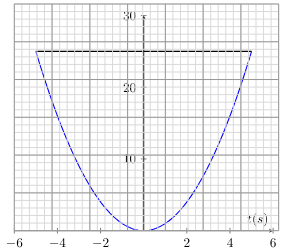
\includegraphics[width=0.3\textwidth]{./img/courbeInc.png}
	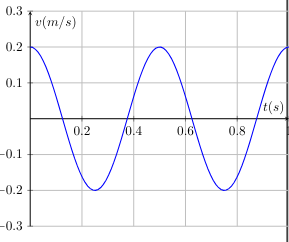
\includegraphics[width=0.3\textwidth]{./img/courbeInc01.png}
  \end{center}
   \end{Box2}

\begin{Box2}{Exercice 9 :Pendule élastique}
   %% \begin{wrapfigure}[12]{r}{0.5\textwidth}
\begin{wrapfigure}[2]{r}{0.3\textwidth}

  \begin{center}
	  \vspace{-0.6cm}
	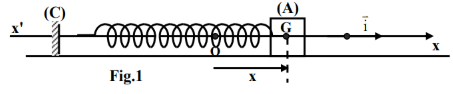
\includegraphics[width=0.3\textwidth]{./img/ex8_00.png}
  \end{center}
\end{wrapfigure}
Un pendule élastique horizontal est constitué par un solide (S) de masse m = 500 g, attaché à l’une des extrémités
d’un ressort horizontal, parfaitement élastique, de raideur K et de masse négligeable par rapport à celle du solide,
l’autre extrémité du ressort étant fixe (figure 1).

  \begin{center}
    \vspace{-0.2cm}
	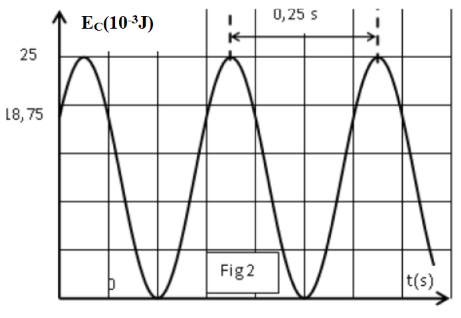
\includegraphics[width=0.4\textwidth]{./img/ex_8_01.png}
  \end{center}

	  \vspace{-1cm}
On néglige tout type de frottement et on étudie le mouvement du solide (S) relativement à un repère galiléen
     $(O, \vec{i})$ horizontal, d’origine O coincidant avec la position d’équilibre du centre d’inertie du solide.
On écarte le solide (S) de sa position d’équilibre d’une distance Xm puis on le lˆache sans vitesse.
     Lorsque le solide passe par sa position d’abscisse $x_0(x_0 != 0)$ avec une vitesse initiale $v_0$ $(v_0 != 0)$ en se dirigeant
dans le sens positif, on déclenche le chronomètre (c’est l’instant $t = 0s$ ) pour commencer l’étude du mouvement.

\begin{enumerate}
  \item  En appliquant la 2eme  loi de Newton au solide (S), tablir l’équation difféerentielle de son mouvement.
Quelle est la nature de ce mouvement?

\item Montrer que $x(t) = X_m sin (\omega_0t + \omega_x)$ est une solution de l’éequation différentielle précédente à condition
que la pulsation $\omega_0$ vérifie une expression qu’on donnera en fonction de K et m.
Donner l’expression de la période propre $T_0$ des oscillations du solide (S).
\item Déduire l’expression de la vitesse du solide en fonction de $X_m$, $\omega_0$, $t$ et $\phi_x$
\item Montrer que $x_0$ et $v_0$ vérifient la relation $x_{02} + \frac{v_0^2}{\omega_0^2} = X_m^2$
\item Un ordinateur muni d’une interface et d’un capteur a enregistrée les variations de l’énergie cinétique du solide
(S) au cours du temps t, le graphe obtenu sur l’écran de l’ordinateur est donné par la figure 2.
\begin{enumerate}
  \item Donner l’expression de l’éenergie mécanique E du système $S_0 = {(S)+ ressort }$ en fonction de x, v, K
et m avec x élongation du solide (S) et v sa vitesse à un instant t quelconque.
\item Montrer que l’énergie E est constante puis donner son expression en fonction de m et $V_m$; $V_m$ amplitude
de la vitesse $v$ du solide.
\item Etablir l’expression de l’énergie cinétique du solide (S) en fonction $m$, $V_m$, $\omega_0$, $t$ et $\phi$. Montrer qu’on
  peut l’écrire sous la forme : $$E_c  = \frac{E_{cmax}}{2}(1 + cos(2\omega_0.t + 2\phi_x))$$
\item  En utilisant le graphe, trouver : $V_m$, $T_0$, $X_m$, $\phi_x$ la phase initiale de l'élongation $x(t)$
\item Ecrire la loi horaire du mouvement.
\item Calculer l’abscisse initiale $x_0(x(t = 0))$ du solide (S) dans le repère $(O, \vec{i})$, d´eduire sa vitesse initiale $v_0$.
Dans quel sens débute le mouvement du solide (S) ?
\item Calculer la raideur K du ressort.
\end{enumerate}
\end{enumerate}


   \end{Box2}
\begin{center} \emph{\textbf{“The physical universe and its buzzing machinery, its fantastical scenery.”}}
\end{center}

%\vspace{-0.6cm}
%%%_________________________Exercice 5 : _________________________Exercice
%\begin{Box2}{Exercice 4 : }
   %% \begin{wrapfigure}[14]{r}{0.5\textwidth}
  %%\begin{center}
	  %%\vspace{-0.6cm}
	%%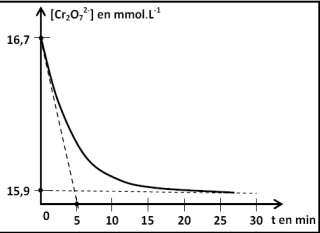
\includegraphics[width=0.5\textwidth]{./img/ex5.png}
  %%\end{center}
%%\end{wrapfigure}

%4

%\end{Box2}

%\begin{Box2}{Exercice 5 : }

%44
%\end{Box2}


%\begin{Box2}{Exercice 6 : }


	%\end{Box2}


%\begin{Box2}{Exercice 7 : }
%\end{Box2}
\end{document}
